\chapter{Resultados}
	
	\section{Análisis de datos de las variables climáticas propuestas}
	
	Los datos utilizados fueron obtenidos de \textit{NASA Langley Research Center (LaRC) POWER Project} financiado por el Programa de Ciencias de la Tierra/Ciencias Aplicadas de la NASA.
	
		\subsection{Radiación solar de onda corta}
			
			En la~\cref{fig:SFC_SW_DWN} observamos que de marzo a septiembre tenemos los niveles más altos de \acrlong{roc}.
	
			\begin{figure}[H]
				\centering
				\begin{subfigure}[t]{0.45\linewidth}
					\centering
					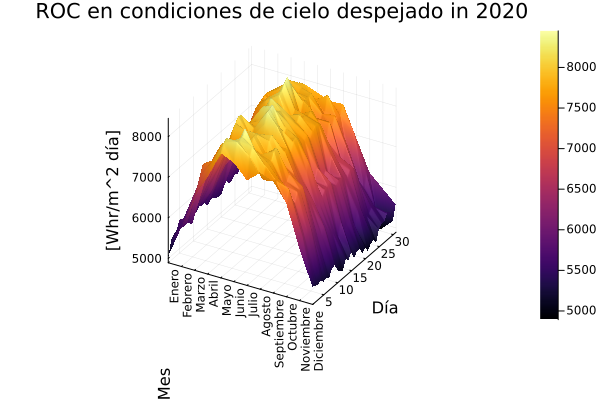
\includegraphics[
						width=\linewidth,
						height = 60mm,
						keepaspectratio
					]{Resultados/DataAnalysis/CLRSKY_SFC_SW_DWN_surface_2020_3d.png}
					\caption{Irradiación de onda corta total recibida por día en condiciones de cielo despejado durante el 2020 sobre el lugar seleccionado}
					\label{fig:CLRSKY_SFC_SW_DWN_surface_2020_3d}
				\end{subfigure}
				\hfill
				\begin{subfigure}[t]{0.45\linewidth}
					\centering
					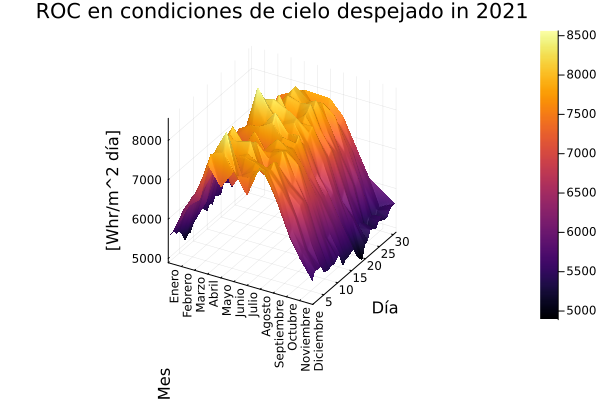
\includegraphics[
						width=\linewidth,
						height = 60mm,
						keepaspectratio
					]{Resultados/DataAnalysis/CLRSKY_SFC_SW_DWN_surface_2021_3d.png}
					\caption{Irradiación de onda corta total recibida por día en condiciones de cielo despejado durante el 2021 sobre el lugar seleccionado}
					\label{fig:CLRSKY_SFC_SW_DWN_surface_2021_3d}
				\end{subfigure}
			\end{figure}
			
			\begin{figure}[H]\ContinuedFloat
				\begin{subfigure}[t]{0.45\linewidth}
					\centering
					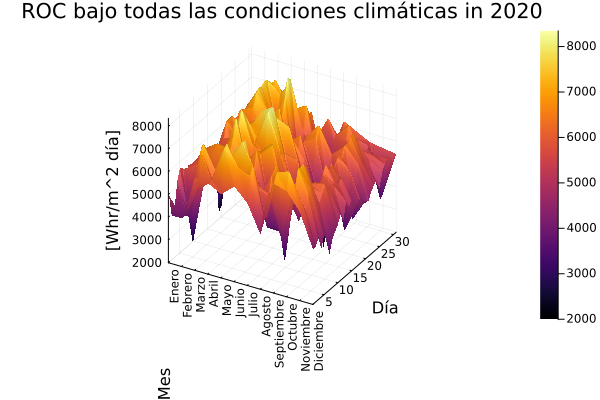
\includegraphics[
						width=\linewidth,
						height = 60mm,
						keepaspectratio
					]{Resultados/DataAnalysis/ALLSKY_SFC_SW_DWN_surface_2020_3d.png}
					\caption{Irradiación de onda corta total recibida por día bajo todas las condiciones climáticas durante el 2020 sobre el lugar seleccionado}
					\label{fig:ALLSKY_SFC_SW_DWN_surface_2020_3d}
				\end{subfigure}
				\hfill
				\begin{subfigure}[t]{0.45\linewidth}
					\centering
					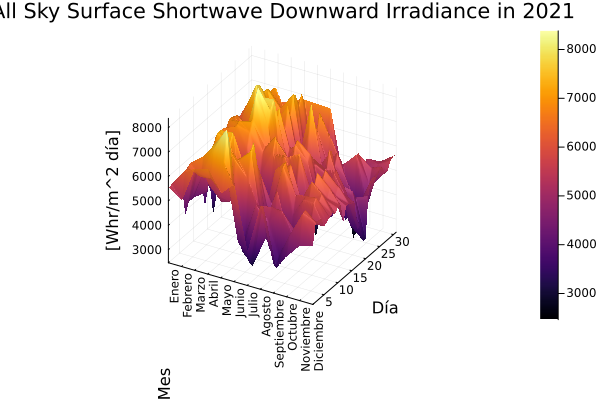
\includegraphics[
						width=\linewidth,
						height = 60mm,
						keepaspectratio
					]{Resultados/DataAnalysis/ALLSKY_SFC_SW_DWN_surface_2021_3d.png}
					\caption{Irradiación de onda corta total recibida por día bajo todas las condiciones climáticas durante el 2021 sobre el lugar seleccionado}
					\label{fig:ALLSKY_SFC_SW_DWN_surface_2021_3d}
				\end{subfigure}
			\end{figure}
			
			\begin{figure}[H]\ContinuedFloat
				\begin{subfigure}[t]{0.45\linewidth}
					\centering
					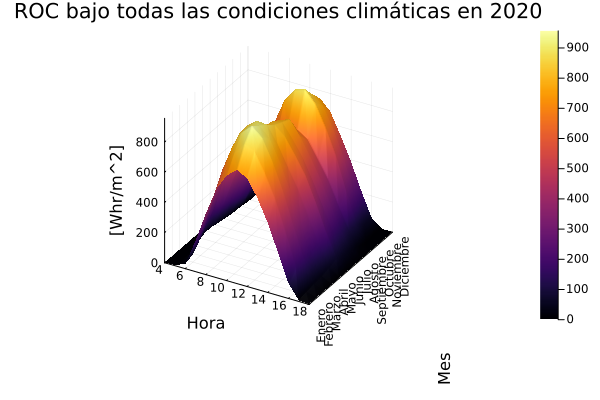
\includegraphics[
						width=\linewidth,
						height = 60mm,
						keepaspectratio
					]{Resultados/DataAnalysis/ALLSKY_SFC_SW_DWN_3d_mean_2020.png}
					\caption{Irradiación de onda corta promedio recibida por hora bajo todas las condiciones climáticas durante el 2020 sobre el lugar seleccionado}
					\label{fig:ALLSKY_SFC_SW_DWN_3d_mean_2020}
				\end{subfigure}
				\hfill
				\begin{subfigure}[t]{0.45\linewidth}
					\centering
					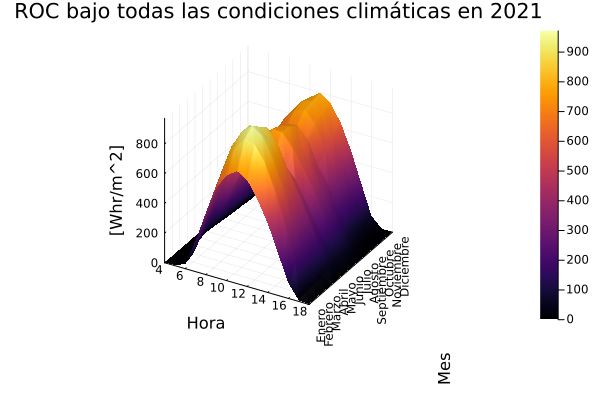
\includegraphics[
						width=\linewidth,
						height = 60mm,
						keepaspectratio
					]{Resultados/DataAnalysis/ALLSKY_SFC_SW_DWN_3d_mean_2021.png}
					\caption{Irradiación de onda corta promedio recibida por hora bajo todas las condiciones climáticas durante el 2021 sobre el lugar seleccionado}
					\label{fig:ALLSKY_SFC_SW_DWN_3d_mean_2021}
				\end{subfigure}
				\caption{Irradiación de onda corta recibida en el lugar físico de experimentación durante 2020 y 2021}
				\label{fig:SFC_SW_DWN}
			\end{figure}

		\subsection{Temperatura}
			
			\begin{figure}[H]
				\centering
				\begin{subfigure}[t]{\linewidth}
					\centering
					\includegraphics[
						width=\linewidth,
						height=70mm,
						keepaspectratio
					]{Resultados/DataAnalysis/Temperatura-promedio-por-hora-en-Ciudad-de-México.png}
					\\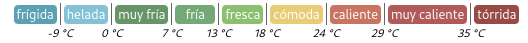
\includegraphics[
						width=0.8\linewidth,
						keepaspectratio
					]{Resultados/DataAnalysis/WeatherSpark-Temperatura-Leyenda.png}
					\caption{Temperatura promedio por hora en Ciudad de México}
					\label{fig:Temperatura-promedio-por-hora-en-Ciudad-de-México}
				\end{subfigure}
			\end{figure}
			\begin{figure}\ContinuedFloat
				\begin{subfigure}[t]{\linewidth}
					\centering
					\includegraphics[
						width=\linewidth,
						height=70mm,
						keepaspectratio
					]{Resultados/DataAnalysis/Temperatura-por-hora-en-2022-Ciudad-de-México.png}\\
					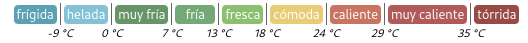
\includegraphics[
						width=0.8\linewidth,
						keepaspectratio
					]{Resultados/DataAnalysis/WeatherSpark-Temperatura-Leyenda.png}
					\caption{Temperatura por hora del 2022 en la Ciudad de México}
					\label{fig:Temperatura-por-hora-en-2022-Ciudad-de-México}
				\end{subfigure}
				\caption{Mapas de temperaturas de la Ciudad de México}
				\floatfoot{Los gráficos fueron obtenidos de \href{https://es.weatherspark.com/y/5674/Clima-promedio-en-Ciudad-de-México-México-durante-todo-el-año}{\textcopyright WeatherSpark.com}}
				\label{fig:Temperatura-CDMX}
			\end{figure}
		
		\section{Presión atmosférica}
			
			\begin{figure}[H]
				\centering
				\begin{subfigure}[t]{0.45\linewidth}
					\centering
					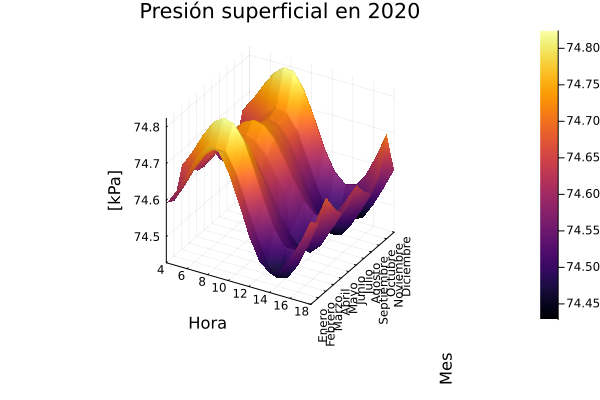
\includegraphics[
						width=\linewidth,
						height = 60mm,
						keepaspectratio
					]{Resultados/DataAnalysis/PS_3d_mean_2020.png}
					\caption{Presión promedio por hora del viento durante 2020 sobre el lugar seleccionado}
					\label{fig:PS_3d_mean_2020}
				\end{subfigure}
				\hfill
				\begin{subfigure}[t]{0.45\linewidth}
					\centering
					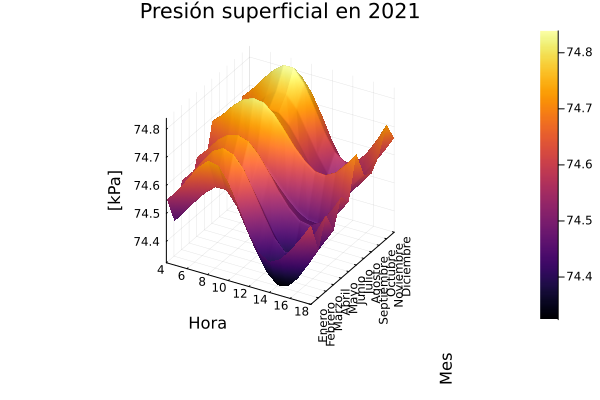
\includegraphics[
						width=\linewidth,
						height = 60mm,
						keepaspectratio
					]{Resultados/DataAnalysis/PS_3d_mean_2021.png}
					\caption{Presión promedio por hora del viento durante 2021 sobre el lugar seleccionado}
					\label{fig:PS_3d_mean_2021}
				\end{subfigure}
				\caption{Presión promedio en el lugar físico de experimentación durante 2020 y 2021}
				\label{fig:PS_3d_mean}
			\end{figure}
			
		\section{Magnitud del perfil de velocidad del viento}
			
			\begin{figure}[H]
				\centering
				\begin{subfigure}[t]{0.45\linewidth}
					\centering
					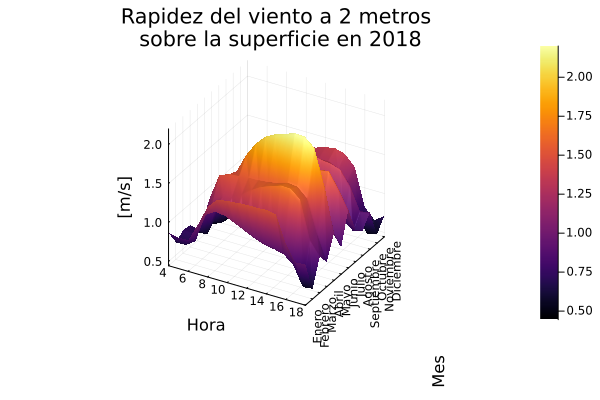
\includegraphics[
						width=\linewidth,
						height = 60mm,
						keepaspectratio
					]{Resultados/DataAnalysis/WS2M_3d_mean_2018.png}
					\caption{Rapidez promedio por hora del viento durante 2018 sobre el lugar seleccionado}
					\label{fig:WS2M_3d_mean_2018}
				\end{subfigure}
				\hfill
				\begin{subfigure}[t]{0.45\linewidth}
					\centering
					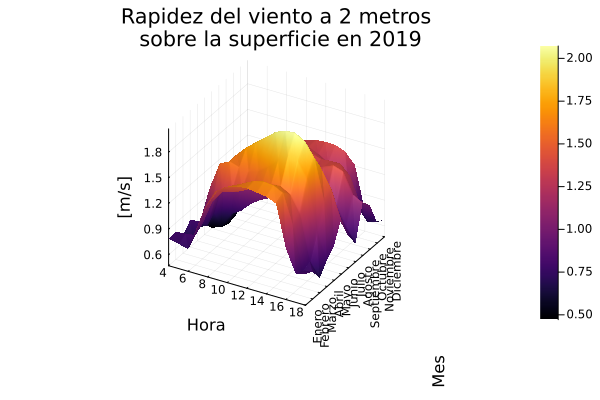
\includegraphics[
						width=\linewidth,
						height = 60mm,
						keepaspectratio
					]{Resultados/DataAnalysis/WS2M_3d_mean_2019.png}
					\caption{Rapidez promedio por hora del viento durante 2019 sobre el lugar seleccionado}
					\label{fig:WS2M_3d_mean_2019}
				\end{subfigure}
			\end{figure}
			
			\begin{figure}[H]\ContinuedFloat
				\begin{subfigure}[t]{0.45\linewidth}
					\centering
					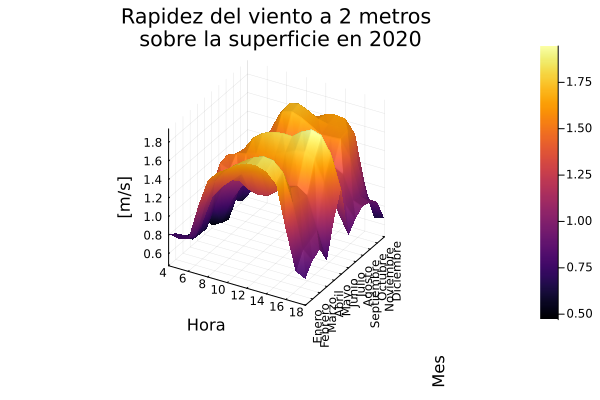
\includegraphics[
						width=\linewidth,
						height = 60mm,
						keepaspectratio
					]{Resultados/DataAnalysis/WS2M_3d_mean_2020.png}
					\caption{Rapidez promedio por hora del viento durante 2020 sobre el lugar seleccionado}
					\label{fig:WS2M_3d_mean_2020}
				\end{subfigure}
				\hfill
				\begin{subfigure}[t]{0.45\linewidth}
					\centering
					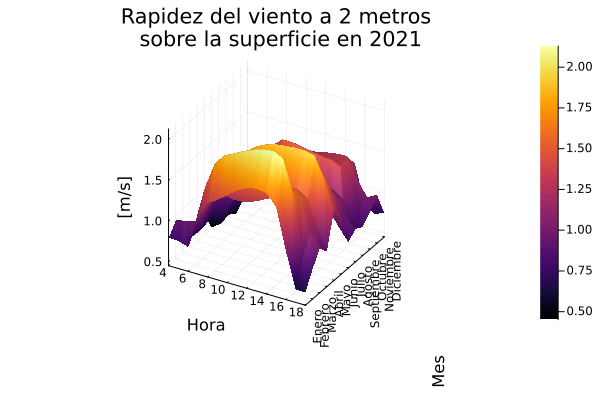
\includegraphics[
						width=\linewidth,
						height = 60mm,
						keepaspectratio
					]{Resultados/DataAnalysis/WS2M_3d_mean_2021.png}
					\caption{Rapidez promedio del viento durante 2021 sobre el lugar seleccionado}
					\label{fig:WS2M_3d_mean_2021}
				\end{subfigure}
				\caption{Rapidez promedio por hora del viento sobre el lugar seleccionado}
				\label{fig:WS2M_3d_mean}
			\end{figure}
	
	\section{Definición de parámetros de salida del agua}
		
		Usando los límites de operación encontrados del análisis de datos se calcula mediante \eqref{equ:interpolación-lineal-simple} y los datos de los~\cref{ch:seawater-properties,ch:agua-saturada-propiedades} la temperatura de ebullición del agua de mar en el sitio de experimentación y a la cual se le agrega un \percent{2} de tolerancia.
		
		\begin{equation}\label{equ:interpolación-lineal-simple}
			y = y_{0} + \dfrac{y_{1}-y_{0}}{x_{1}-x_{0}} \times (x-x_{0})
		\end{equation}
		
		\begin{longtblr}[
			caption = {Datos a interpolar para definir los parámetros de salida del agua},
			label = {table:interpolación-agua-salida},
		]{
			colspec = {*{3}{X}},
			hlines,
			vlines,
			row{odd} = {bg=tablerowblue},
			row{1} = {
				bg = tabletitleblue,
				fg=white,
				font = \bfseries
			},
			width=0.75\linewidth,
			rowhead = 1,
			rows={
				valign = m,
				halign = c,
				mode = math
			}
		}
			~ & y & x\\
			0 & \qty{90}{\degreeCelsius} & \qty{70.14}{\kilo\pascal}\\
			1 & \qty{95}{\degreeCelsius} & \qty{80.55}{\kilo\pascal}\\
			\text{T}_{\text{salida}} & ~ & \qty{74.80}{\kilo\pascal}
		\end{longtblr}
		
		\begin{align*}
			\text{T}_{\text{ebullición agua dulce}} &= \qty{90}{\degreeCelsius} + \dfrac{\qty{95}{\degreeCelsius} - \qty{90}{\degreeCelsius}}{\qty{80.55}{\kilo\pascal}-\qty{70.14}{\kilo\pascal}} \times (\qty{74.80}{\kilo\pascal} - \qty{70.14}{\kilo\pascal})\\
			\text{T}_{\text{salida}} &= (\text{T}_{\text{ebullición agua dulce}} + \qty{0.601}{\degreeCelsius}) + \text{Tolerancia}\\
			\text{T}_{\text{salida}} &= (\qty{92.238}{\degreeCelsius} + \qty{0.601}{\degreeCelsius}) \times (1.02)\\
			\text{T}_{\text{salida}} &\approx \qty{94.70}{\degreeCelsius}
		\end{align*}
		
		Y considerando una temperatura mínima de entrada del agua igual a \qty{13}{\degreeCelsius} tenemos calculamos mediante \eqref{equ:potencia-necesaria-agua} el flujo de calor necesario por unidad de flujo másico que se necesita para lograr la ebullición del agua y el cambio de fase.
		
		\begin{equation}\label{equ:potencia-necesaria-agua}
			\dfrac{\dot{Q}}{\dot{m}} = \left(\gls{cs}_{\text{agua}} \Delta T + \gls{hl}\right)
		\end{equation}
		
		Para conocer $\gls{cs}_{\text{agua}}$ de la \cref{table:Calor-específico-agua} se usa \eqref{equ:interpolación-lineal-simple} para obtener el calor específico estimado a los \qty{13}{\degreeCelsius} y a los \qty{94.7}{\degreeCelsius}.
		
		\begin{align*}
			\gls{cs}_{13} &= \qty{3968.1}{\joule\per\kg\kelvin} + \dfrac{\qty{3973.4}{\joule\per\kg\kelvin} - \qty{3968.1}{\joule\per\kg\kelvin}}{\qty{20}{\degreeCelsius}-\qty{10}{\degreeCelsius}} \times (\qty{20}{\degreeCelsius} - \qty{13}{\degreeCelsius})\\
			\gls{cs}_{13} &= \qty{3971.8}{\joule\per\kg\kelvin}\\
			\gls{cs}_{94.7} &= \qty{4010.5}{\joule\per\kg\kelvin} + \dfrac{\qty{4019.9}{\joule\per\kg\kelvin} - \qty{4010.5}{\joule\per\kg\kelvin}}{\qty{100}{\degreeCelsius}-\qty{90}{\degreeCelsius}} \times (\qty{100}{\degreeCelsius} - \qty{94.7}{\degreeCelsius})\\
			\gls{cs}_{94.7} &= \qty{4015.5}{\joule\per\kg\kelvin}
		\end{align*}
		
		Una vez obtenidos sacamos el promedio incluyendo el resto del intervalo dándonos que:
		\begin{equation*}
			\gls{cs}_{\text{agua}} = \qty{3989.5}{\joule\per\kg\kelvin}
		\end{equation*}
		
		Similarmente para obtener \gls{hl} aplicamos \eqref{equ:interpolación-lineal-simple} en \cref{table:Calor-latente-vaporización} para obtener la entalpía de vaporización a los \qty{94.7}{\degreeCelsius}.
		
		\begin{align*}
			\gls{hl} &= \qty{2191.3}{\kilo\joule\per\kg} + \dfrac{\qty{2166.2}{\kilo\joule\per\kg} - \qty{2191.3}{\kilo\joule\per\kg}}{\qty{100}{\degreeCelsius}-\qty{90}{\degreeCelsius}} \times (\qty{100}{\degreeCelsius} - \qty{94.7}{\degreeCelsius})\\
			\gls{hl} &= \qty{2178.0}{\kilo\joule\per\kg}
		\end{align*}
		
		Sustituyendo en \eqref{equ:potencia-necesaria-agua} obtenemos que el flujo de calor necesario por unidad de flujo másico es:
		
		\begin{equation}\label{equ:potencia-necesaria-sistema}
			\dot{Q} = \dot{m}\left[\qty{3.9895}{\kilo\joule\per\kg\kelvin} \left(\qty{94.7}{\degreeCelsius}-\qty{13}{\degreeCelsius}\right) + \qty{2178.0}{\kilo\joule\per\kg}\right] = \dot{m} \times \qty{2503.94}{\kilo\joule\per\kg}
		\end{equation}
		
%		
%		Conductividad térmica
%		
%		Para conocer $\gls{cs}_{\text{agua}}$ de la \cref{table:Conductividad-térmica-agua-salada} se usa \eqref{equ:interpolación-lineal-simple} para obtener la conductividad estimada a los \qty{13}{\degreeCelsius} y a los \qty{94.7}{\degreeCelsius}.
%		
%		\begin{align*}
%			\gls{cs}_{13} &= \qty{0.586}{\watt\per\m\kelvin} + \dfrac{\qty{0.601}{\watt\per\m\kelvin} - \qty{0.586}{\watt\per\m\kelvin}}{\qty{20}{\degreeCelsius}-\qty{10}{\degreeCelsius}} \times (\qty{20}{\degreeCelsius} - \qty{13}{\degreeCelsius})\\
%			\gls{cs}_{13} &= \qty{0.591}{\watt\per\m\kelvin}\\
%			\gls{cs}_{94.7} &= \qty{0.670}{\watt\per\m\kelvin} + \dfrac{\qty{0.674}{\watt\per\m\kelvin} - \qty{0.670}{\watt\per\m\kelvin}}{\qty{100}{\degreeCelsius}-\qty{90}{\degreeCelsius}} \times (\qty{100}{\degreeCelsius} - \qty{94.7}{\degreeCelsius})\\
%			\gls{cs}_{94.7} &= \qty{0.672}{\watt\per\m\kelvin}
%		\end{align*}
%		
%		Una vez obtenidos sacamos el promedio incluyendo el resto del intervalo dándonos que:
%		\begin{equation*}
%			\gls{cs}_{\text{agua}} = \qty{0.638}{\watt\per\m\kelvin}
%		\end{equation*}